\begin{figure}
\centering
  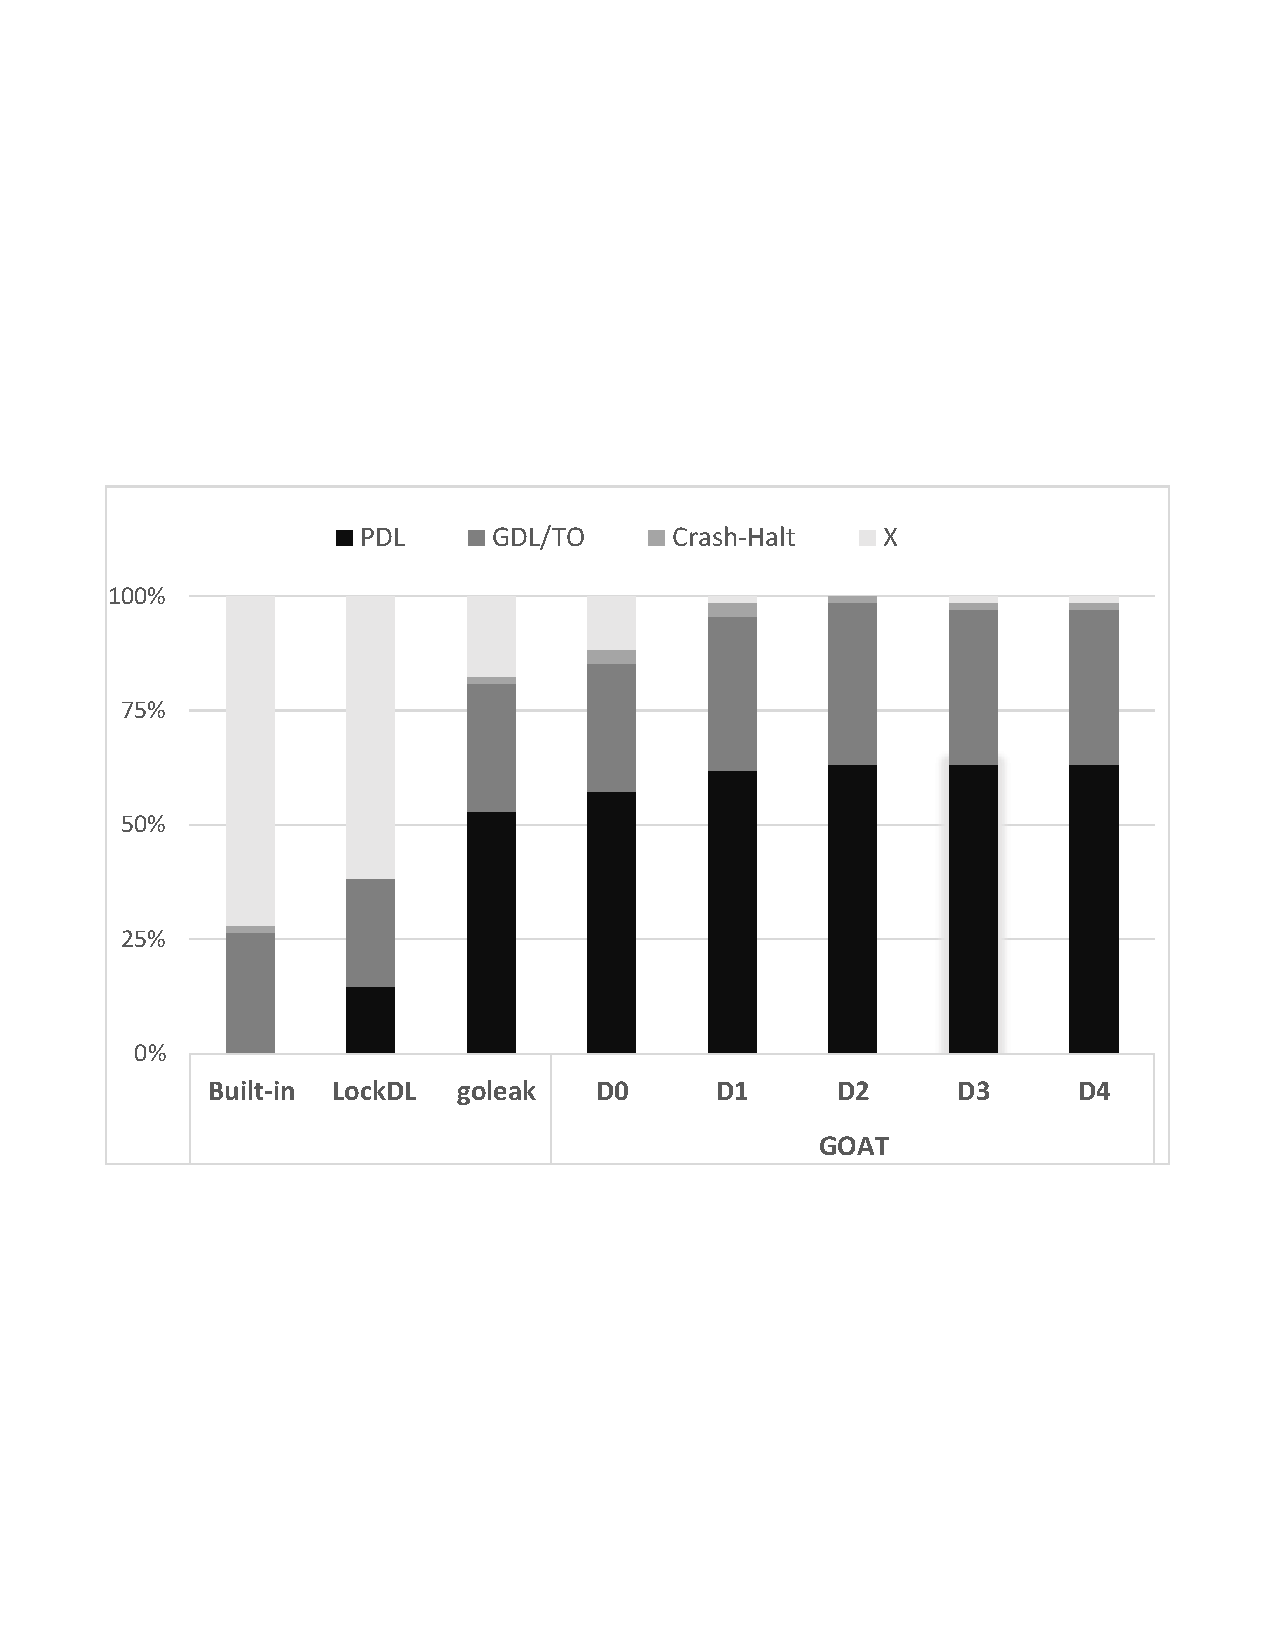
\includegraphics[width=.95\linewidth]{figs/P4_detections.pdf}
  \caption{Distribution of detected bugs by built-in deadlock detector (BUILTINDL), LockDL, GoLeak, and GOAT different D over 1000 runs. PDL: partial deadlock, GDL/TO: global deadlock, Crash/Halt: causes the program to crash or halt during detection, X: nothing is detected }
  \label{fig:detection}
\end{figure}


\begin{figure}
\centering
  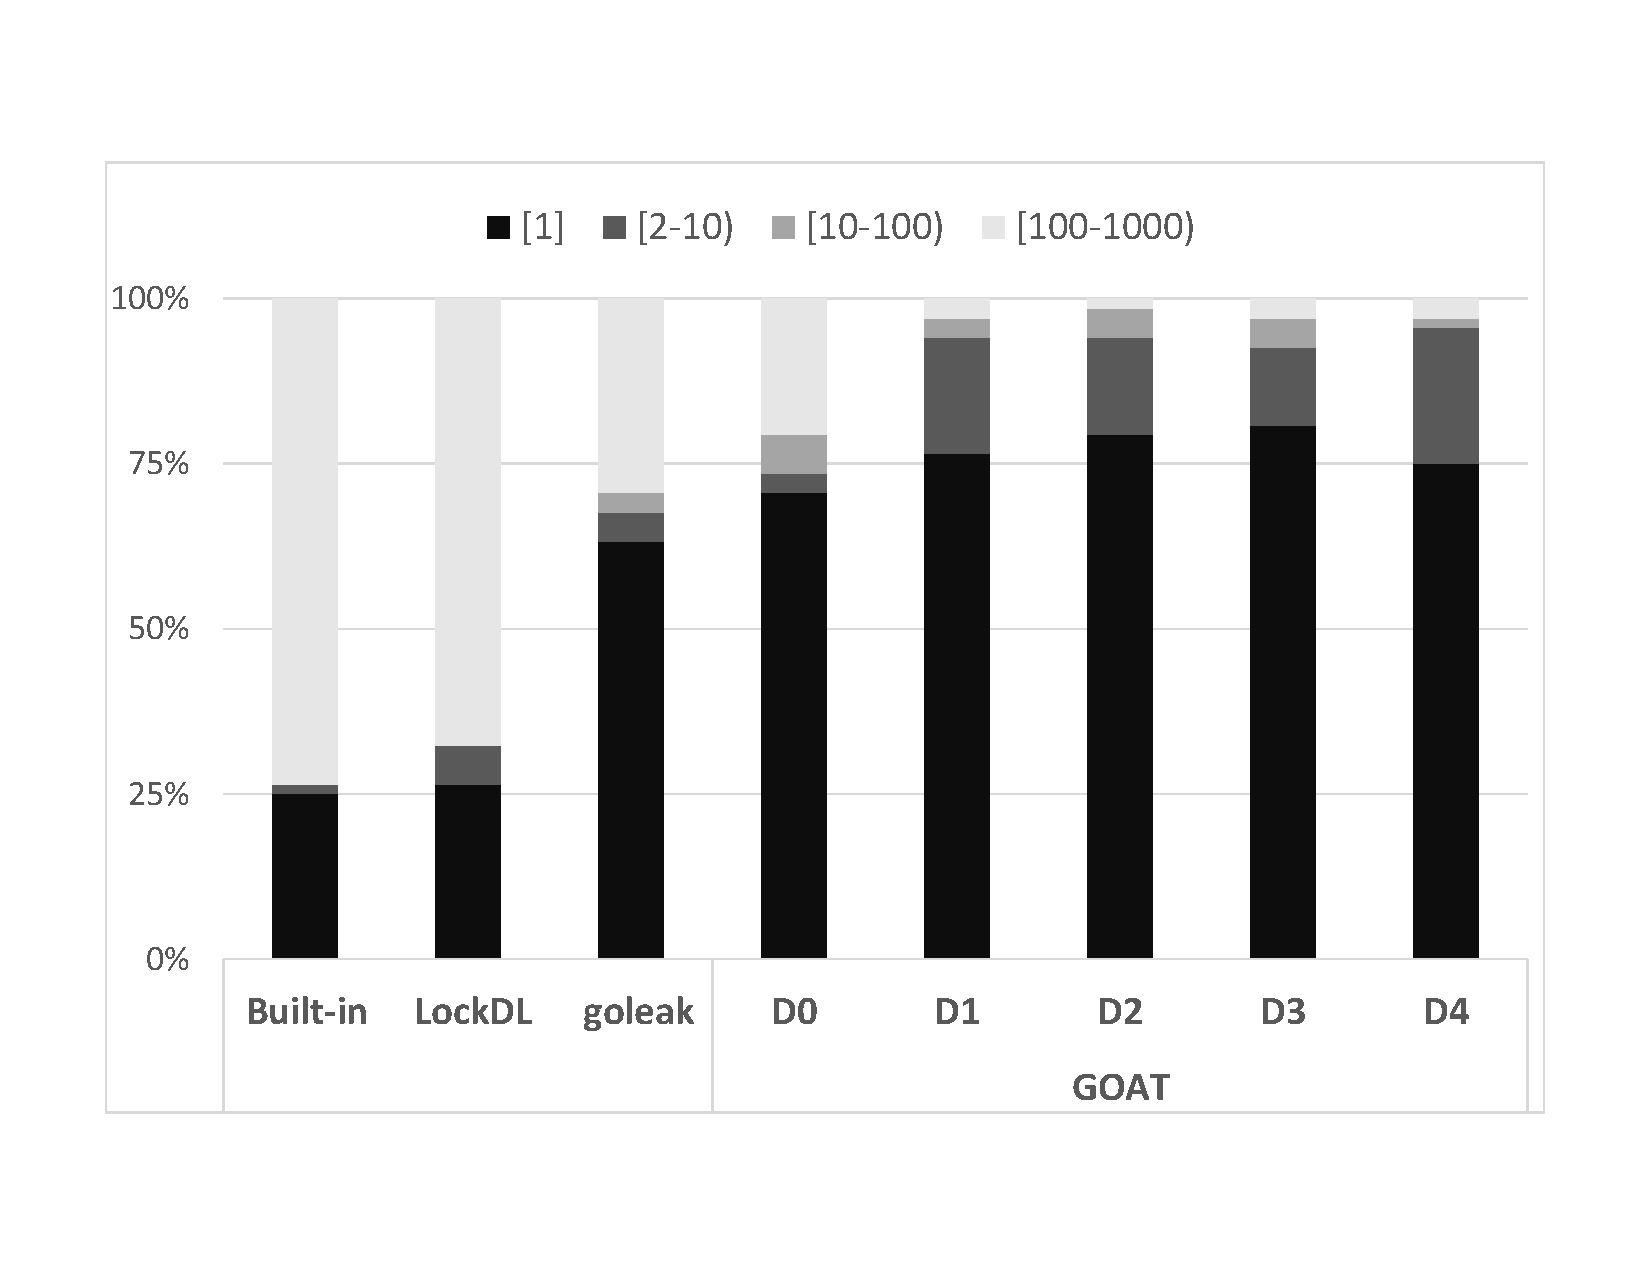
\includegraphics[width=.95\linewidth]{figs/P4_runs.pdf}
  \caption{Distribution of required number of iterations to detect the bug for each tool}
  \label{fig:runs}
\end{figure}

\subsection{Deadlock Detection}
\label{sec:dl_evaluation}
We assess the ability of \goat and its variations in detecting bugs with minimum number of executions required to expose the bug.
%
We have compared \goat against three existing dynamic detectors:
\begin{itemize}
  \item \textit{Built-in} deadlock detector: It is an embeded mechanism in the standard Go runtime. The mechanism periodically makes sure that the queue of \textit{runnable} goroutines is never empty until the main goroutine terminates. If the queue is empty and main has not terminated yet (\ie main is blocked), it throws a runtime error.
  \item \textit{goleak} \cite{goleak}: This leak detector from Uber checks the program stack at the end of the main goroutine's execution to find the application-level goroutines that remained in the stack (\ie leaked).
  \item \textit{LockDL} \cite{lockdl}: This tool intercept with all mutex locks and unlocks of the target application to maintain a ``lock-set'' data structure. \textit{LockDL} issues warning during runtime when it finds a circular wait in the lock-set or double-locking the same lock. It has a timeout mechanism for application that traps into global deadlocks (30 seconds by default).
\end{itemize}

\stcmtside{fix}
All experiments are performed on a server with two AMD Ryzen 5 3600 6-Core Processor (12 total cores with 2 threads per core and 6 cores per socket), 64 GB of RAM with generic Ubuntu 4.15.0 and Go version 1.15.6.
%
Table \ref{tab:comparison} shows the details of results obtained from executing each tool per bug 1000 times.
%
We show that the tool is unable to detect the bug after 1000 executions with \textbf{X (1000)}.
%

%
Figure \ref{fig:detection} and table \ref{tab:comparison} show that variations of \goat outperforms other detector by discovering the bug in 100\% of the GoKer blocking benchmark.
%
Figure \ref{fig:runs} and highlighted cells of table \ref{tab:comparison} show that the idea of injecting random delays around concurrency usage points in the program drastically reduces the required number of testing iterations until the bug occur.
%
D0 means \goat did not delay the program at any point and D4 means that the target program has been delayed up to four times around its CU points.
%
Figures \ref{fig:detection} and \ref{fig:runs} also state that the increase in the delay bound of \goat does not necessarily increase the chance of exposing the bug.
%
For example, the row of bug \texttt{serving\_2137} in table \ref{tab:comparison} show that only \goat D2 were able to detect the bug.


\begin{figure}
\centering
  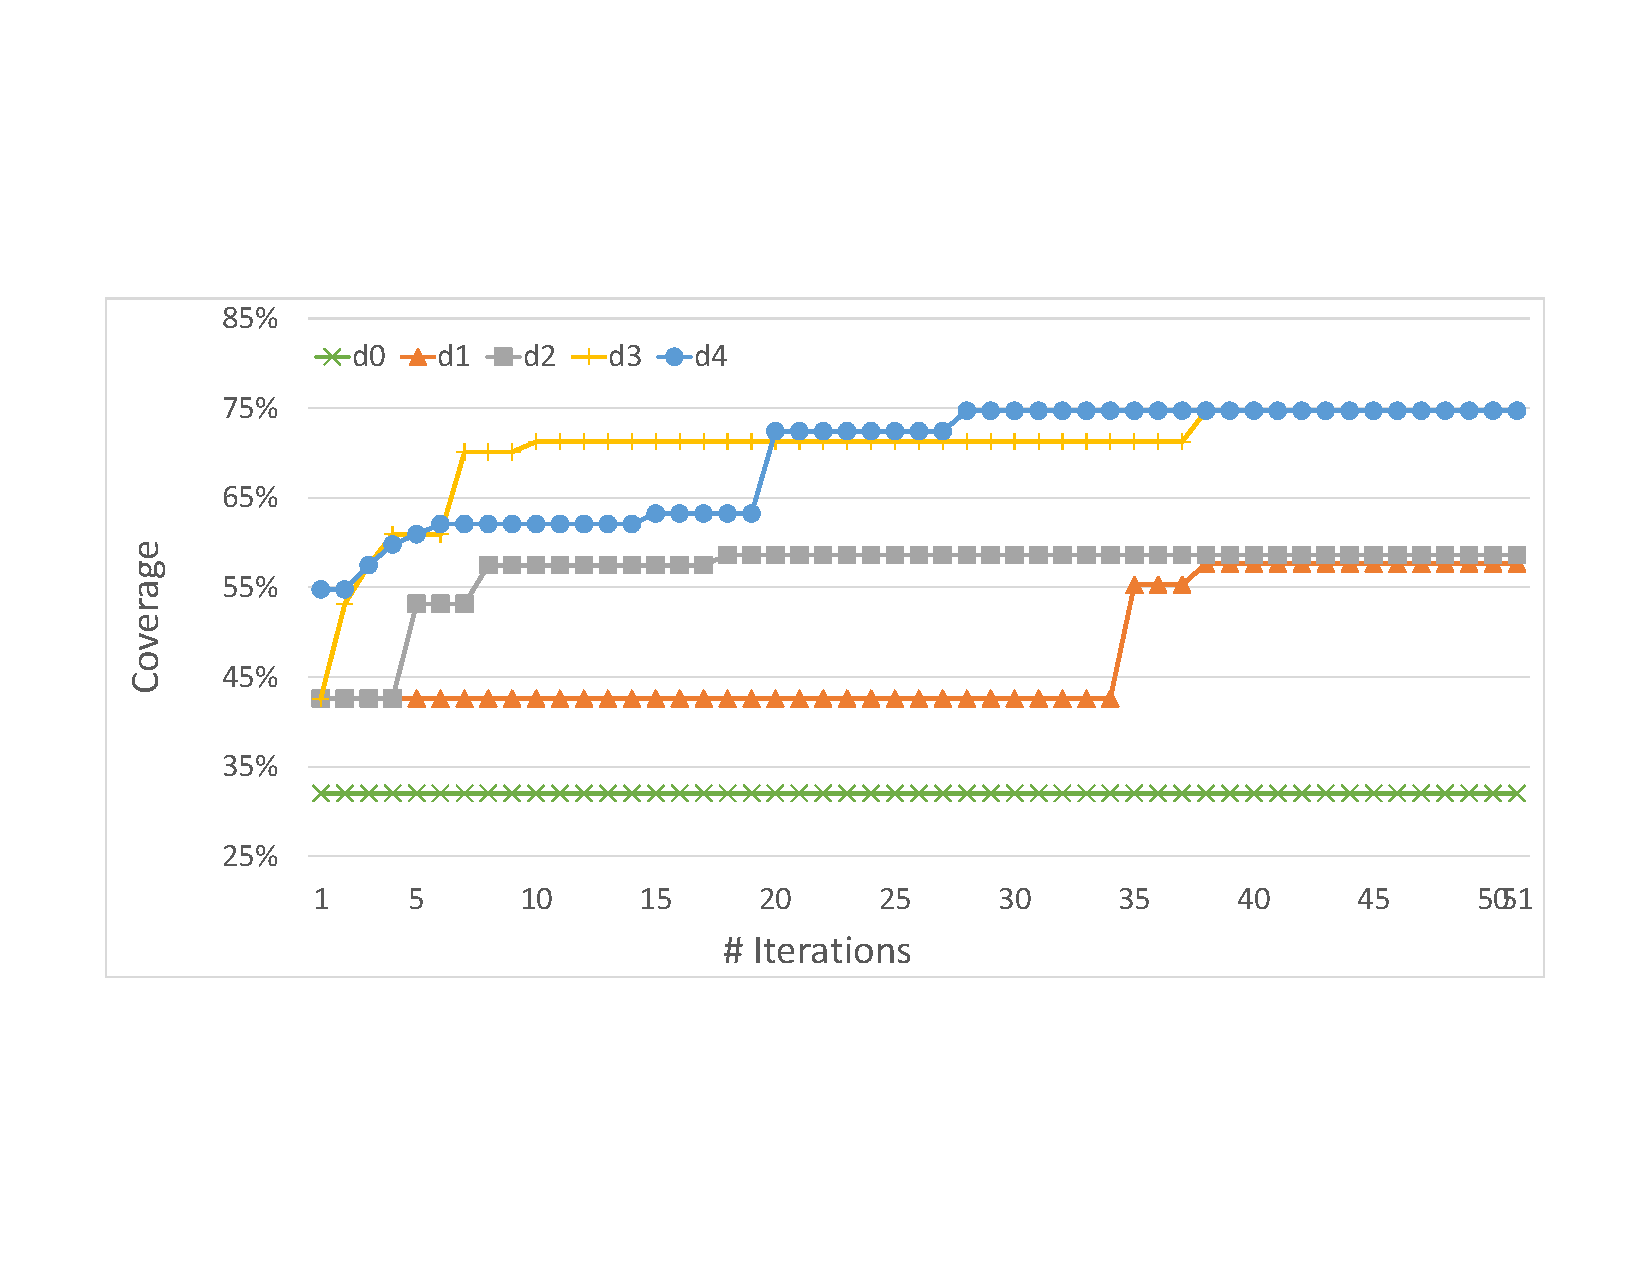
\includegraphics[width=.95\linewidth]{figs/coverage_etcd7443.pdf}
  \caption{etcd7442 coverage}
  \label{fig:etcd_coverage}
\end{figure}


\begin{figure}
\centering
  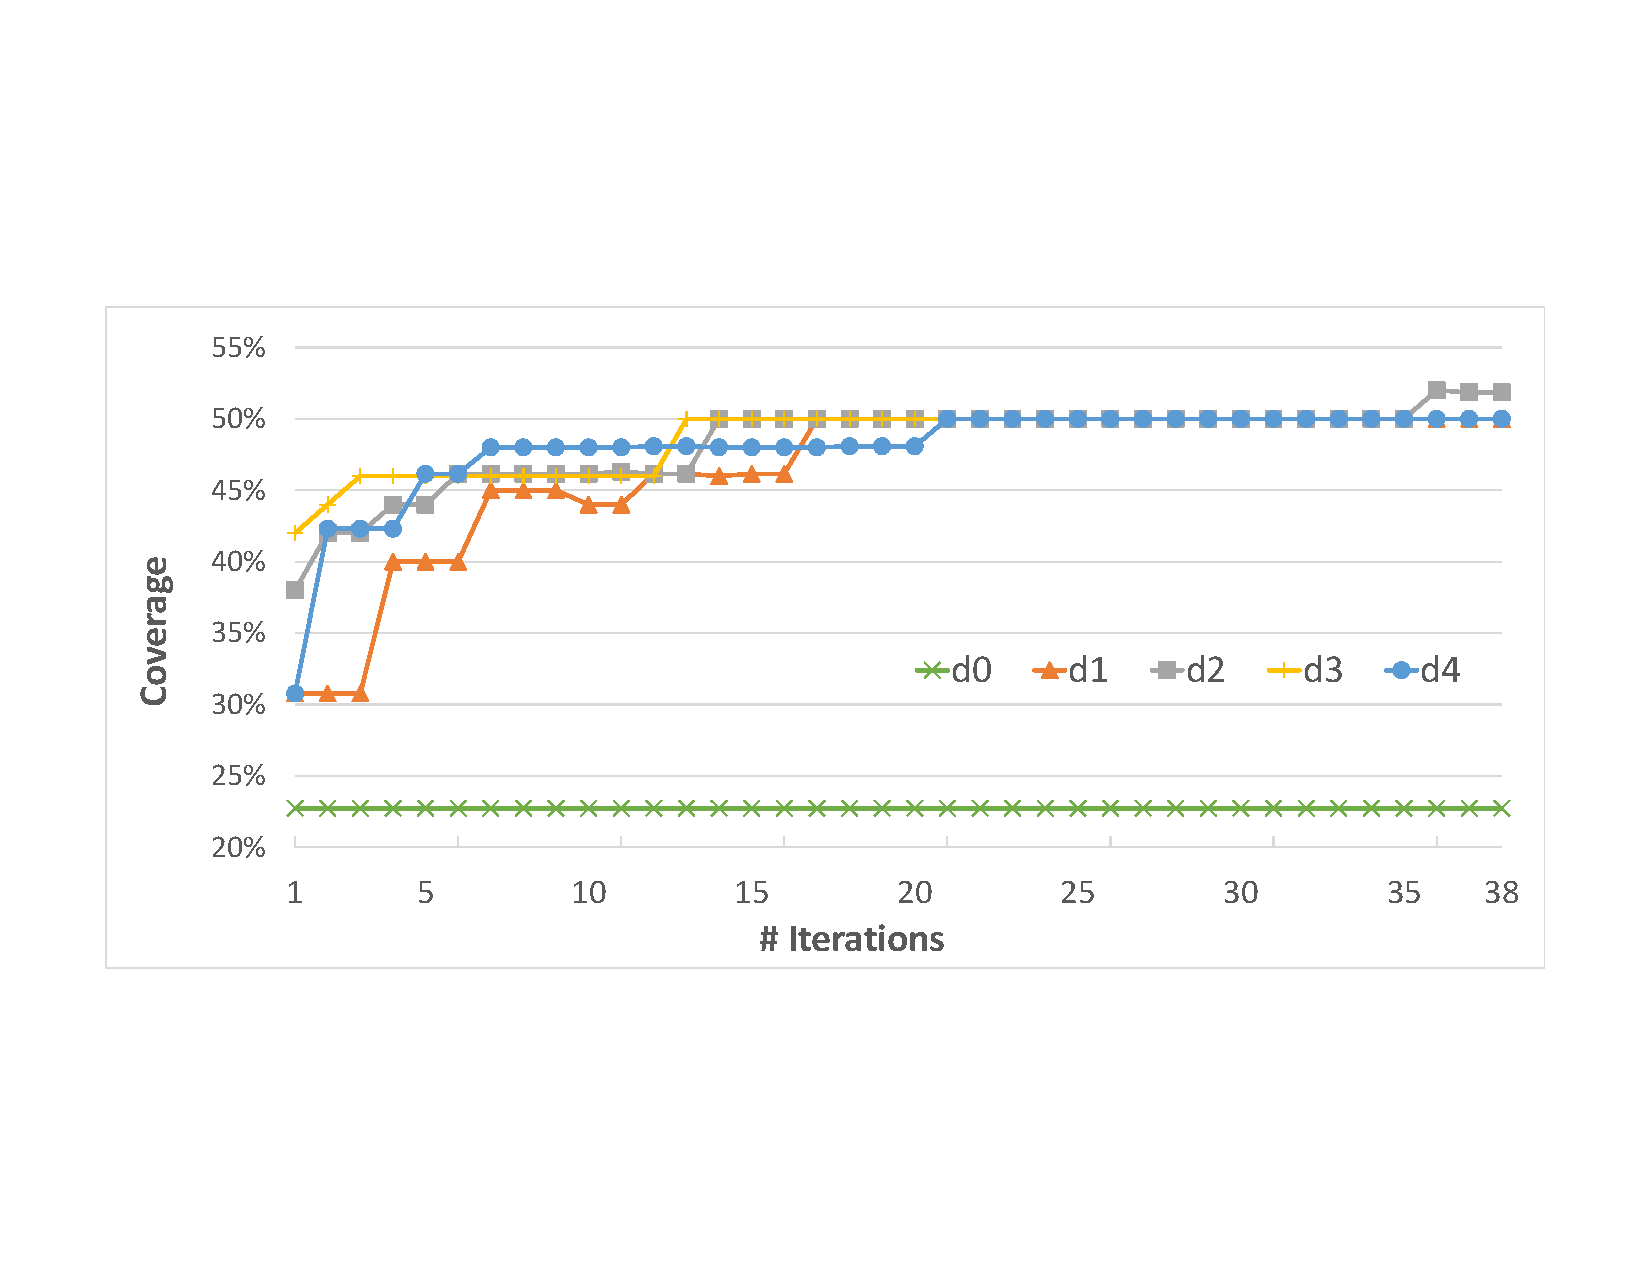
\includegraphics[width=.95\linewidth]{figs/coverage_kubernetes11298.pdf}
  \caption{kuberenetes11298 coverage}
  \label{fig:kubernetes_coverage}
\end{figure}

\subsection{Coverage Analyis}
We picked two representative bug kernels \texttt{etcd7443} and \texttt{kubernetes11298} to evaluate the coverage idea on them as they
%
both have extensive use of channels, mutexes, conditional variables, nested selects within nested for loops and the buggy interleaving is proved to be rare to happen.
%
figures \ref{fig:etcd_coverage} and \ref{fig:kubernetes_coverage} show the gradual increase in coverage percentage during execution runs for different values of D.
%
Recall that D is the bound on the number of yields that we inject to the native execution of a given program to perturb the scheduler around concurrency usages.
%
These figures show that the increase of number of delays grows the rate of coverage percentage.
%
However, higher number of delays do not necessarily increase the coverage (D2 and D4 in figure \ref{fig:kubernetes_coverage}).
%
The drop in coverage for D1 in figure \ref{fig:kubernetes_coverage} is because of the new coverage requirements (\eg, a new goroutine is spawned and executing some concurrency primitives) that were encountered during testing execution.
